\documentclass[compress]{beamer}

\usetheme[block=fill]{metropolis}

\usepackage{graphicx} % Allows including images
\usepackage{amsmath,amsfonts,amsthm,amssymb}
\usepackage{color}
\usepackage{xcolor,cancel}
%\usepackage{enumitem}
%\setitemize{label=\usebeamerfont*{itemize item}%
%	\usebeamercolor[fg]{itemize item}
%	\usebeamertemplate{itemize item}}
\definecolor{mDarkBrown}{HTML}{604c38}
\definecolor{mDarkTeal}{HTML}{23373b}
\definecolor{mLightBrown}{HTML}{EB811B}
\definecolor{mMediumBrown}{HTML}{C87A2F}
\definecolor{mygreen}{HTML}{98C2B9}
\definecolor{myyellow}{HTML}{DFD79C}
\definecolor{myblue}{HTML}{8CA7CC}
\definecolor{kern}{HTML}{8CC2B7}


\usepackage{float}
\usepackage{framed}
\usepackage{epsfig}
\usepackage{graphicx}
\usepackage{subcaption}
\usepackage{ulem}
\usepackage{hhline}
\usepackage{multirow}
\usepackage{comment}   
\usepackage{bbm}
\usepackage{tikz}   
\def\Put(#1,#2)#3{\leavevmode\makebox(0,0){\put(#1,#2){#3}}}
\newcommand*\mystrut[1]{\vrule width0pt height0pt depth#1\relax}
\newcommand{\eqdef}{\mathbin{\stackrel{\rm def}{=}}}


\newcommand{\bs}[1]{\boldsymbol{#1}}
\newcommand{\bv}[1]{\mathbf{#1}}
\newcommand{\R}{\mathbb{R}}
\newcommand{\E}{\mathbb{E}}

\DeclareMathOperator*{\argmin}{arg\,min}
\DeclareMathOperator*{\argmax}{arg\,max}
\DeclareMathOperator{\nnz}{nnz}
\DeclareMathOperator{\diag}{diag}
\DeclareMathOperator{\Var}{Var}
\DeclareMathOperator{\vol}{vol}
\DeclareMathOperator{\sinc}{sinc}
\DeclareMathOperator{\sign}{sign}
\DeclareMathOperator{\dist}{dist}
\DeclareMathOperator{\mv}{mv}
\DeclareMathOperator{\sgn}{sgn}
\DeclareMathOperator{\step}{step}
\DeclareMathOperator{\gap}{gap}
\DeclareMathOperator{\poly}{poly}
\DeclareMathOperator{\tr}{tr}
\DeclareMathOperator{\orth}{orth}
\newcommand{\norm}[1]{\|#1\|}
\captionsetup[subfigure]{labelformat=empty}
\captionsetup[figure]{labelformat=empty}
\DeclareMathOperator*{\lmin}{\lambda_{min}}
\DeclareMathOperator*{\lmax}{\lambda_{max}}

\newcommand{\specialcell}[2][c]{%
  \begin{tabular}[#1]{@{}c@{}}#2\end{tabular}}
\newcommand{\specialcellleft}[2][c]{%
\begin{tabular}[#1]{@{}l@{}}#2\end{tabular}
}

\newtheorem{claim}[theorem]{Claim}

\usepackage{tabstackengine}
\stackMath


%----------------------------------------------------------------------------------------
%	TITLE PAGE
%----------------------------------------------------------------------------------------

\title{CS-GY 6763: Lecture 9 \\ Dimension Dependent Optimization}
\author{NYU Tandon School of Engineering, Prof. Christopher Musco}
\date{}

\begin{document}

\begin{frame}
	\titlepage 
\end{frame}

\metroset{titleformat=smallcaps}

\begin{frame}[t]
	\frametitle{administrative}
	\begin{itemize}
		\item Project proposal due \emph{next Wednesday, 11/9}.
		\item Problem set 3 will be released shortly.
		\item We are working grading pset 2 and midterms.
	\end{itemize}
\end{frame}

\begin{frame}[t]
	\frametitle{first order convex optimization}
	\textbf{First Order Optimization:} Given a convex function $f$ and a convex set $\mathcal{S}$, 
	\begin{center}
		\textbf{Goal:} Find $\hat{\bv{x}}\in \mathcal{S}$ such that $f(\hat{\bv{x}}) \leq \min_{\bv{x}\in \mathcal{S}}f(\bv{x})+\epsilon$.
	\end{center}
	Assume we have:
	\begin{itemize}
		\item \textbf{Function oracle}: Evaluate $f(\bv{x})$ for any $\bv{x}$. 
		\item \textbf{Gradient oracle}: Evaluate $\nabla f(\bv{x})$ for any $\bv{x}$.
		\item \textbf{{Projection oracle}}: Evaluate $P_{\mathcal{S}}(\bv{x})$ for any $\bv{x}$.
	\end{itemize}
Gradient descent requires $O\left(\frac{R^2G^2}{\epsilon^2}\right)$ calls to each oracle  to solve the problem. 

We were only able to improve the $\epsilon$ dependence by making stronger assumptions on $f$ (strong convexity, smoothness). 
\end{frame}

\begin{frame}[t]
	\frametitle{dimension dependent bound}
	Alternatively, we can get much better bounds if we are willing to depend on the \emph{problem dimension}. I.e. on $d$ if $f(\bv{x})$ is a function mapping $d$-dimensional vectors to scalars.   
	
	We already know how to do this for a few special functions:
	
	\begin{align*}
		f(\bv{x}) &= \|\bv{A}\bv{x} - \bv{b}\|_2^2 & &\text{where} & \bv{A}&\in \R^{n\times d}.
	\end{align*}
	
\end{frame}

\begin{frame}[t]
	\frametitle{dimension dependent bound}	
	Let $f(\bv{x})$ be bounded between $[-B, B]$ on $\mathcal{S}$. 
	\begin{theorem}[Dimension Dependent Convex Optimization]
		There is an algorithm (the Center-of-Gravity Method) which finds $\hat{\bv{x}}$ satisfying $f(\hat{\bv{x}}) \leq \min_{\bv{x}\in \mathcal{S}}f(\bv{x})+\epsilon$  using $O(d\log(B/\epsilon))$ calls to a function and gradient oracle for $f$.
	\end{theorem}
	\textbf{Caveat:} Assumes we have some representation of $\mathcal{S}$, not just a projection oracle. We will discuss this more later.
	
	\textbf{Note:} For an unconstrained problem with known starting radius $R$, can take $\mathcal{S}$ to be the ball of radius $R$ around $\bv{x}^{(1)}$. If $\max_{\bv{x}}\|\nabla f(\bv{x})\|_2 = G$, we always have $B = O(R G)$. 
	
\end{frame}

\begin{frame}[t]
	\frametitle{center of gravity method}
	\textbf{A few basic ingredients:}

	1. The center-of-gravity of a convex set $\mathcal{S}$ is defined as:
	\begin{align*}
		c = \frac{\int_{x\in \mathcal{S}} x\, dx}{\vol(\mathcal{S})} =  \frac{\int_{x\in \mathcal{S}} x\, dx}{\int_{x\in \mathcal{S}} 1\, dx}
	\end{align*}

	2. For two convex sets $\mathcal{A}$ and $\mathcal{B}$, $\mathcal{A}\cap \mathcal{B}$ is convex. Proof by picture:
\end{frame}

\begin{frame}[t]
	\frametitle{center of gravity method}
	\begin{center}
		Natural ``cutting plane'' method. Developed simultaneous on opposite sides of iron curtain.
	\end{center}
\begin{center}
	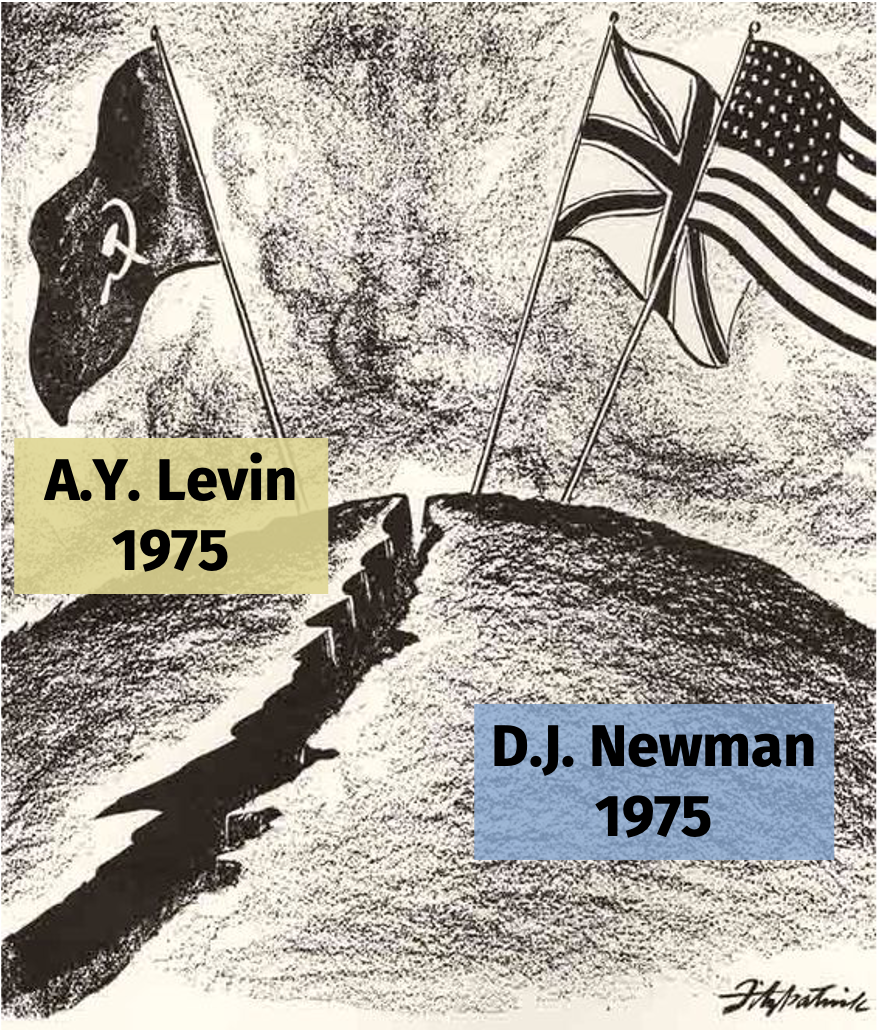
\includegraphics[width=.4\textwidth]{cog_proof.png}
\end{center}

\vspace{-.5em}
Not used in practice (we will discuss why) but the basic idea underlies many algorithms that are. 
\end{frame}

\begin{frame}[t]
	\frametitle{center of gravity method}
	\begin{center}
	Natural ``cutting plane'' method.
	\end{center}
\begin{columns}
	\begin{column}{.6\textwidth}
		\begin{itemize}
			\item $\mathcal{S}_1 = \mathcal{S}$
			\item For $t = 1, \ldots, T:$
			\begin{itemize}
				\item \alert{$\bv{c}_t = \text{center of gravity of } \mathcal{S}_t$.}
				\item Compute $\nabla f(\bv{c}_t)$.
				\item $\mathcal{H} = \{\bv{x} \big\vert \langle \nabla f(\bv{c}_t), \bv{x}-\bv{c}_t\rangle \leq 0\}$.
				\item $\mathcal{S}_{t+1} = \mathcal{S}_{t} \cap H$
			\end{itemize}
			\item Return $\hat{\mathbf{x}} = \argmin_t f(\bv{c}_t)$
		\end{itemize}
	\end{column}
	\begin{column}{.35\textwidth}
	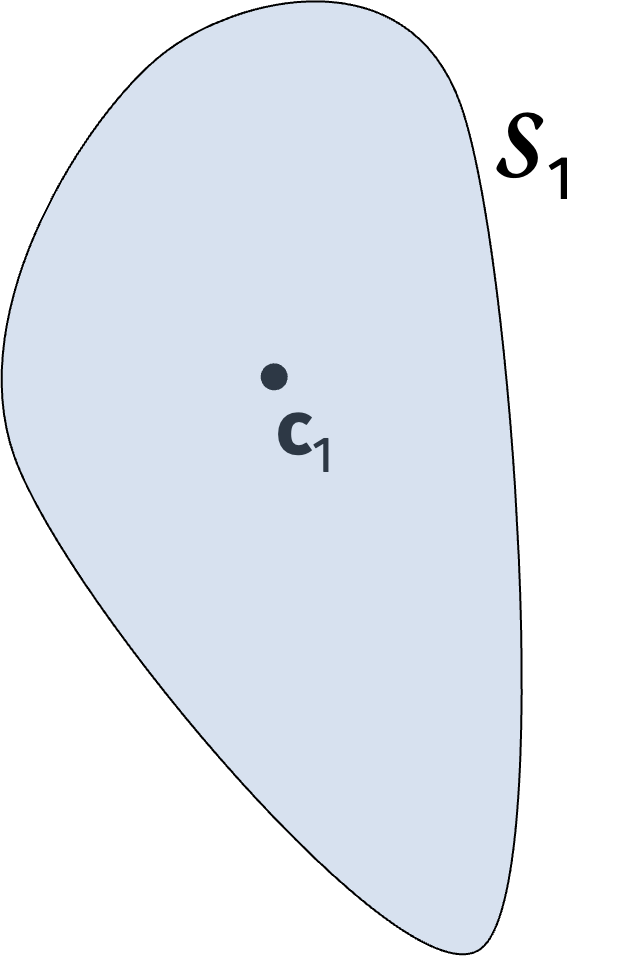
\includegraphics[width=\textwidth]{cog1.png}
\end{column}
\end{columns}
\end{frame}

\begin{frame}[t]
	\frametitle{center of gravity method}
	\begin{center}
		Natural ``cutting plane'' method.
	\end{center}
	\begin{columns}
		\begin{column}{.6\textwidth}
			\begin{itemize}
				\item $\mathcal{S}_1 = \mathcal{S}$
				\item For $t = 1, \ldots, T:$
				\begin{itemize}
					\item $\bv{c}_t = \text{center of gravity of } \mathcal{S}_t$.
					\item \alert{Compute $\nabla f(\bv{c}_t)$.}
					\item $\mathcal{H} = \{\bv{x} \big\vert \langle \nabla f(\bv{c}_t), \bv{x}-\bv{c}_t\rangle \leq 0\}$.
					\item $\mathcal{S}_{t+1} = \mathcal{S}_{t} \cap H$
				\end{itemize}
				\item Return $\hat{\mathbf{x}} = \argmin_t f(\bv{c}_t)$
			\end{itemize}
		\end{column}
		\begin{column}{.35\textwidth}
			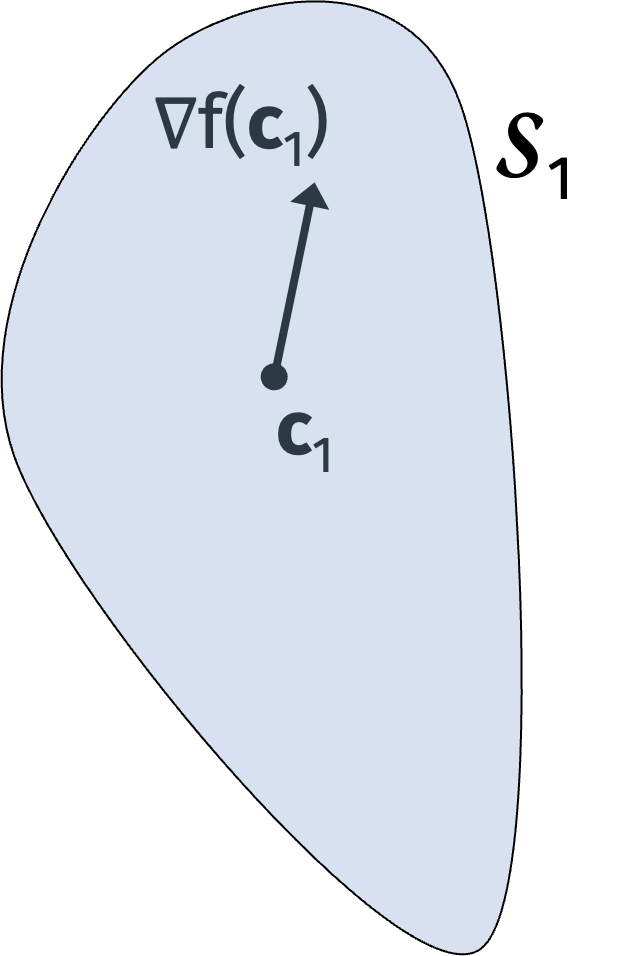
\includegraphics[width=\textwidth]{cog2.png}
		\end{column}
	\end{columns}
\end{frame}

\begin{frame}[t]
	\frametitle{center of gravity method}
	\begin{center}
		Natural ``cutting plane'' method.
	\end{center}
	\begin{columns}
		\begin{column}{.6\textwidth}
			\begin{itemize}
				\item $\mathcal{S}_1 = \mathcal{S}$
				\item For $t = 1, \ldots, T:$
				\begin{itemize}
					\item $\bv{c}_t = \text{center of gravity of } \mathcal{S}_t$.
					\item {Compute $\nabla f(\bv{c}_t)$.}
					\item \alert{$\mathcal{H} = \{\bv{x} \big\vert \langle \nabla f(\bv{c}_t), \bv{x}-\bv{c}_t\rangle \leq 0\}$.}
					\item \alert{$\mathcal{S}_{t+1} = \mathcal{S}_{t} \cap H$}
				\end{itemize}
				\item Return $\hat{\mathbf{x}} = \argmin_t f(\bv{c}_t)$
			\end{itemize}
		\end{column}
		\begin{column}{.6\textwidth}
			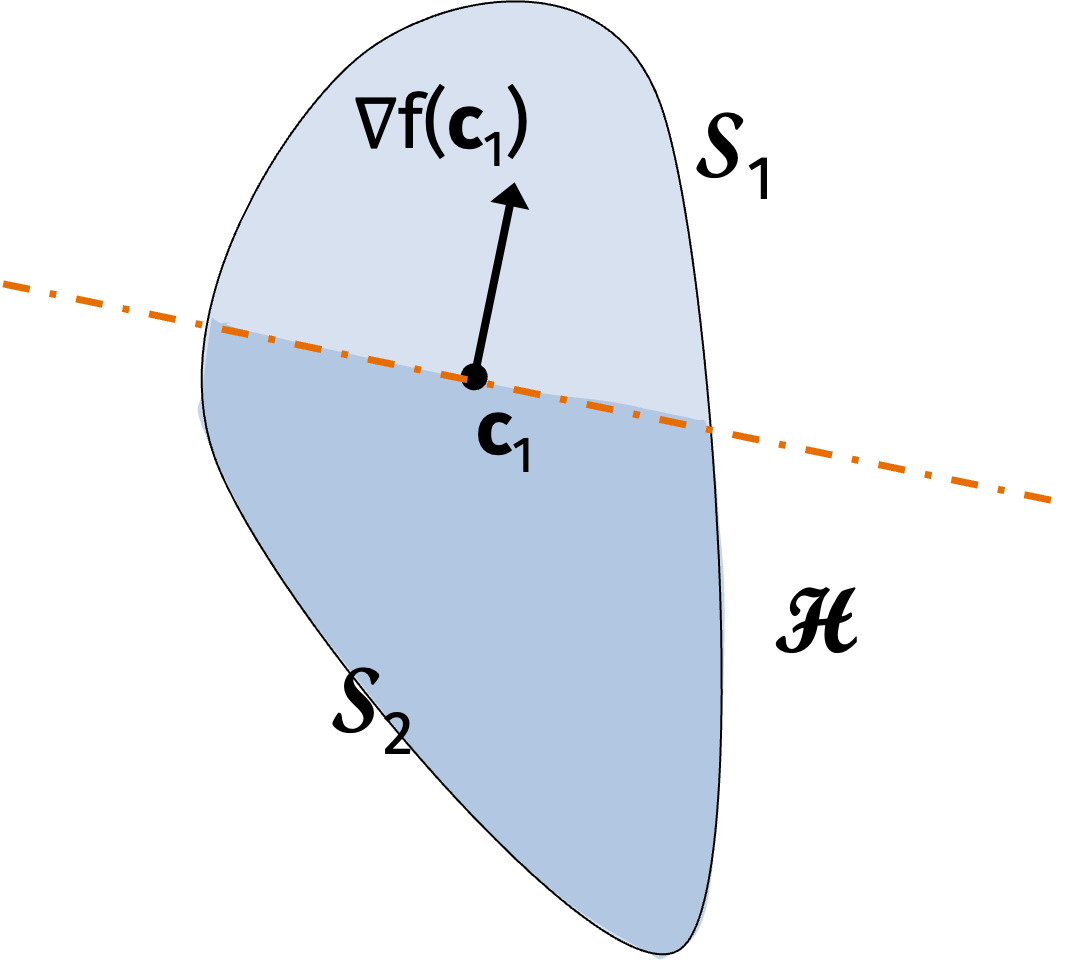
\includegraphics[width=\textwidth]{cog3.png}
		\end{column}
	\end{columns}
\end{frame}

\begin{frame}[t]
	\frametitle{center of gravity method}
	Intuitively, why does it make sense to search in $\mathcal{S}_t \cap \mathcal{H}$ where:
	\begin{align*}
		\mathcal{H} = \{\bv{x} \big\vert \langle \nabla f(\bv{c}_t), \bv{x}-\bv{c}_t\rangle \leq 0\}?
	\end{align*}
	\begin{center}
		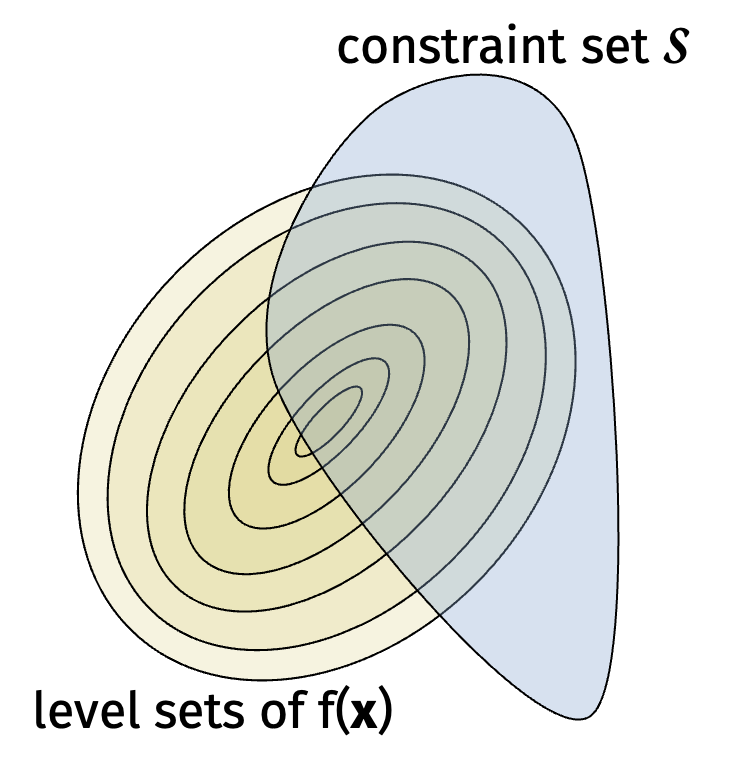
\includegraphics[width=.55\textwidth]{level_sets_constrained.png}
	\end{center}

\end{frame}

\begin{frame}[t]
	\frametitle{center of gravity method}
	Intuitively, why does it make sense to search in $\mathcal{S}_t \cap \mathcal{H}$ where:
	\begin{align*}
		\mathcal{H} = \{\bv{x} \big\vert \langle \nabla f(\bv{c}_t), \bv{x}-\bv{c}_t\rangle \leq 0\}?
	\end{align*}
	
	\begin{columns}
		\begin{column}{.45\textwidth}
			By convexity, if $\bv{y} \notin \{\mathcal{S}_t \cap \mathcal{H}\}$ then:
			\begin{align*}
				f(\bv{y}) &\geq f(\bv{c}_t) +  \langle\nabla f(\bv{c}_t), \bv{y}-\bv{c}_t\rangle\\ &> f(\bv{c}_t)
			\end{align*}
		\end{column}
		\begin{column}{.55\textwidth}
			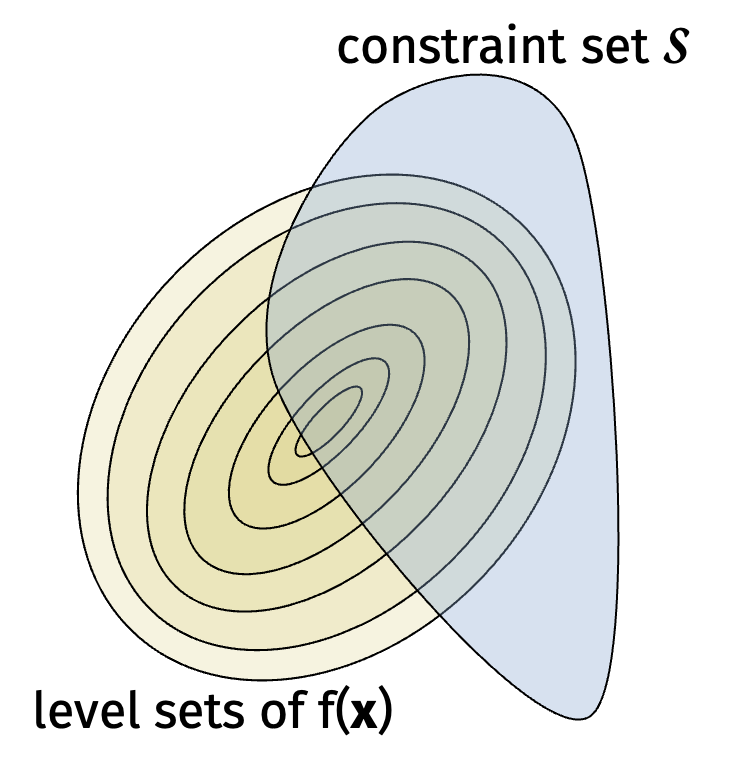
\includegraphics[width=\textwidth]{level_sets_constrained.png}
		\end{column}
	\end{columns}
	
\end{frame}

\begin{frame}[t]
	\frametitle{convergence theorem}
	\begin{theorem}[Center-of-Gravity Convergence]
		Let $f$ be a convex function with values in $[-B,B]$.
		Let $\hat{\bv{x}}$ be the output of the center-of-gravity method run for $T$ iterations. Then:
		\begin{align*}
			f(\hat{\bv{x}}) - f(\bv{x}^*) \leq 2B \left(1-\frac{1}{e}\right)^{T/d} \leq 2B e^{-T/3d}.
		\end{align*}
	\end{theorem}
	If we set $T = 3d\log(2B/\epsilon)$, then $f(\hat{\bv{x}}) - f(\bv{x}^*) \leq \epsilon$. 
\end{frame}

\begin{frame}[t]
	\frametitle{key geometric tool}
	Want to argue that, at every step of the algorithm, we ``cut off'' a large portion of the convex set we are searching over:
	
	\begin{center}
		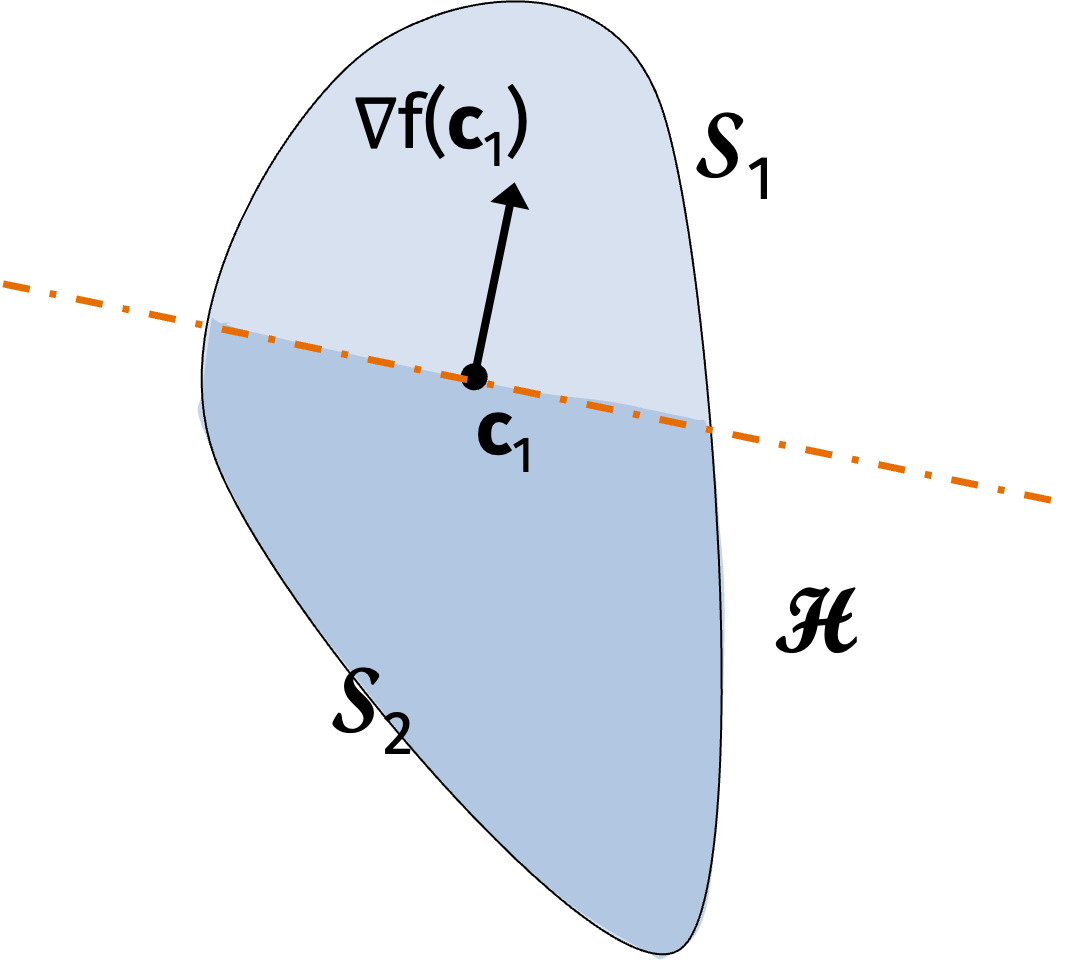
\includegraphics[width=.5\textwidth]{cog3.png}
	\end{center}
\end{frame}

\begin{frame}[t]
	\frametitle{key geometric tool}
	\begin{theorem}[Gr\"{u}nbaum's Theorem]
		For any convex set $\mathcal{S}$ with center-of-gravity $\bv{c}$, and any halfspace 	$\mathcal{Z} = \{\bv{x} \big\vert \langle \bv{a}, \bv{x}-\bv{c}\rangle \leq 0\}$ then:
		\begin{align*}
			\frac{\vol(\mathcal{S} \cap \mathcal{Z})}{\vol(\mathcal{S})}\geq \frac{1}{e} \approx .368
		\end{align*}
	\end{theorem}

\end{frame}

\begin{frame}[t]
	\frametitle{key geometric tool}
	Want to argue that, at every step of the algorithm, we ``cut off'' a large portion of the convex set we are searching over.
	
	\begin{theorem}[Gr\"{u}nbaum's Theorem]
		For any convex set $\mathcal{S}$ with center-of-gravity $\bv{c}$, and any halfspace 	$\mathcal{Z} = \{\bv{x} \big\vert \langle \bv{a}, \bv{x}-\bv{c}\rangle \leq 0\}$ then:
		\begin{align*}
			\frac{\vol(\mathcal{S} \cap \mathcal{Z})}{\vol(\mathcal{S})}\geq \frac{1}{e} \approx .368
		\end{align*}
	\end{theorem}
	
	Let $\mathcal{Z}$ be the compliment of $\mathcal{H}$ from the algorithm. Then we cut off at least a $1/e$ fraction of the convex body on every iteration.  
	
	\textbf{Corollary:} After $t$ steps, $\vol(\mathcal{S}_t) \leq \left(1-\frac{1}{e}\right)^t\vol(\mathcal{S})$.
\end{frame}

\begin{frame}
	\frametitle{convergence proof}
	Let $\delta$ be a small parameter to be chosen later. 
	
	Let $\mathcal{S}^{\delta} = \{(1-\delta)\bv{x}^* + \delta\bv{x} \hspace{.2em}\big\vert \hspace{.2em} \text{for } \bv{x}\in \mathcal{S} \}$.
	
	\begin{center}
	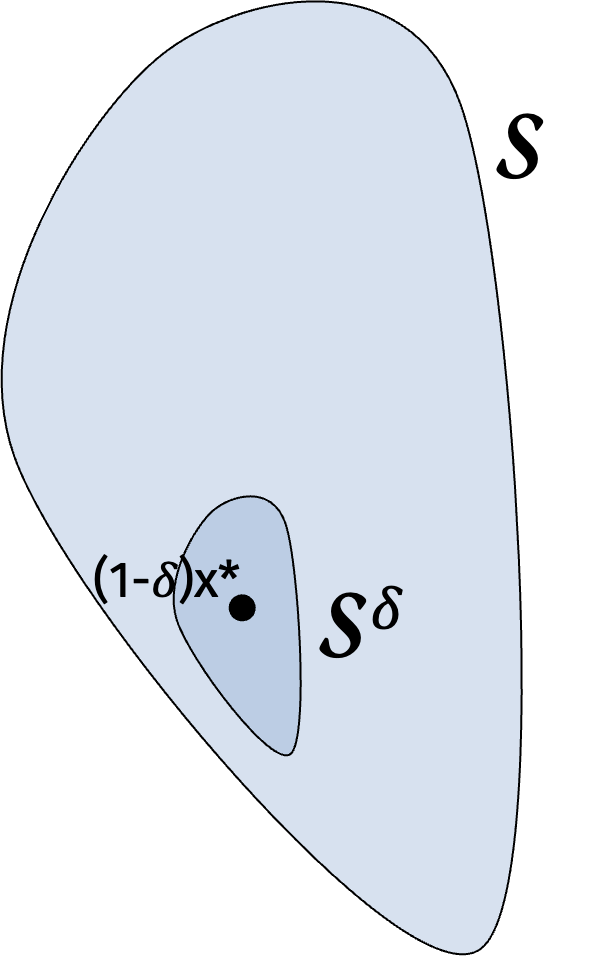
\includegraphics[width=.3\textwidth]{smallbody.png}
	\end{center}
	\textbf{Claim:} Every point $\bv{y}$ in $\mathcal{S}^{\delta}$ has good function value.
\end{frame}
\begin{frame}
	\frametitle{convergence proof}
	\begin{columns}
		\begin{column}{.3\textwidth}
		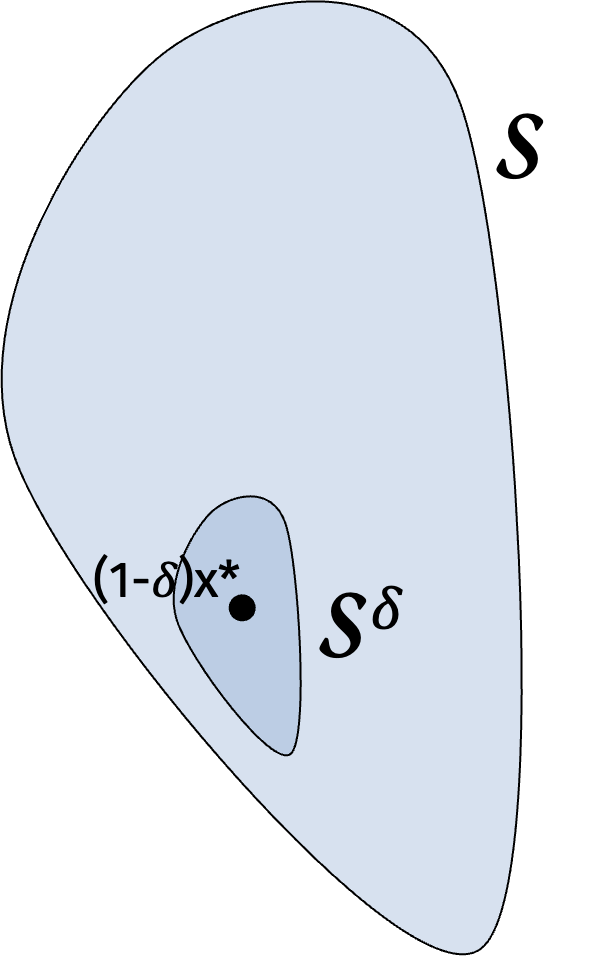
\includegraphics[width=\textwidth]{smallbody.png}
		\end{column}
		\begin{column}{.7\textwidth}
		For any $\bv{y} \in \mathcal{S}^\delta$:	
		\begin{align*}
			f(\bv{y}) &= f\left((1-\delta)\bv{x}^* + \delta \bv{x}\right) \\
			&\leq (1-\delta) f(\bv{x}^*) + \delta f(\bv{x})\\
			& \leq f(\bv{x}^*) - \delta f(\bv{x}^*)  + \delta f(\bv{x})\\
			&\leq f(\bv{x}^*)  + 2B\delta.
		\end{align*}
	\end{column}
	\end{columns}
\end{frame}

\begin{frame}
	\frametitle{convergence proof}
	\begin{columns}
		\begin{column}{.4\textwidth}
			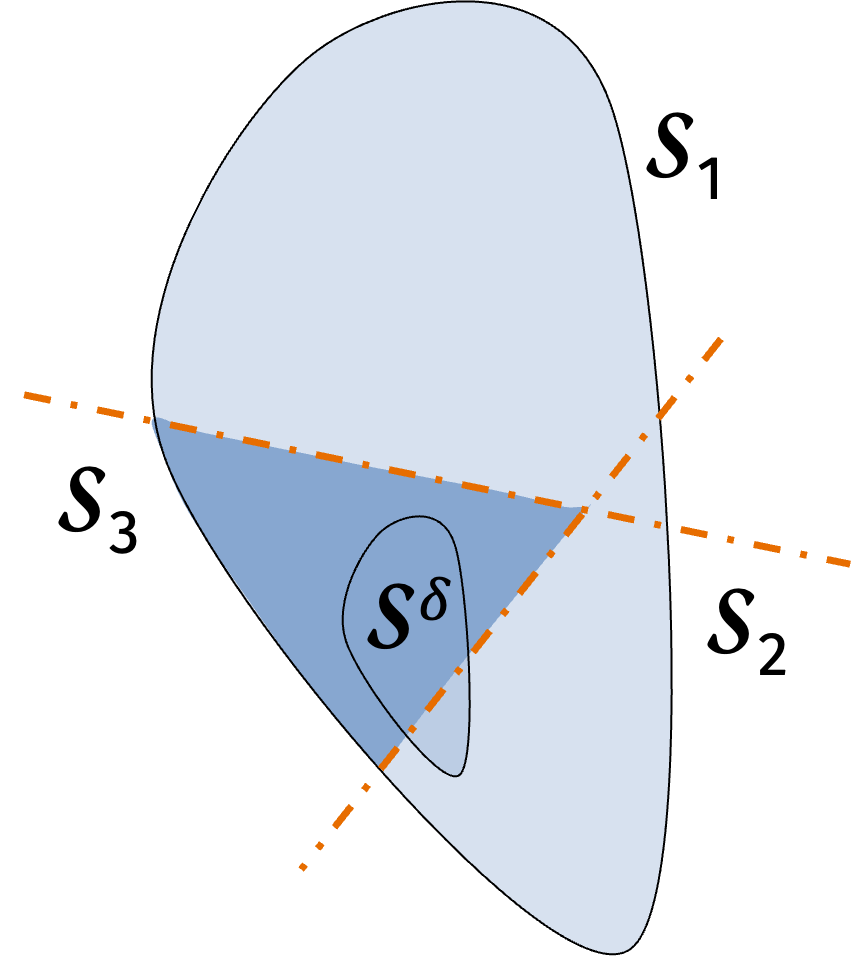
\includegraphics[width=\textwidth]{cut_off.png}
		\end{column}
		\begin{column}{.6\textwidth}
			\vspace{.5em}
			
			We also have: $\vol(\mathcal{S}^\delta) = \delta^d \vol(\mathcal{S}).$
			
			\vspace{1em}
			Set $\delta = \left(1-\frac{1}{e}\right)^{T/d}$. After $T$ steps, $\vol(\mathcal{S}_t) \leq \vol(\mathcal{S}^\delta)$.  
			
			\vspace{1em}
			Either $S_T$ exactly equals $S^{\delta}$, in which case our current centroid gives error $\leq 2B\delta$.
			
			\vspace{1em} Or we must have ``chopped off'' at least one point $\bv{y}$ in $\mathcal{S}^\delta$ by the time we reach step $T$. 
			\vspace{1em}
			
		\end{column}
	\end{columns}
\end{frame}

\begin{frame}
	\frametitle{convergence proof}
	\begin{columns}
		\begin{column}{.4\textwidth}
			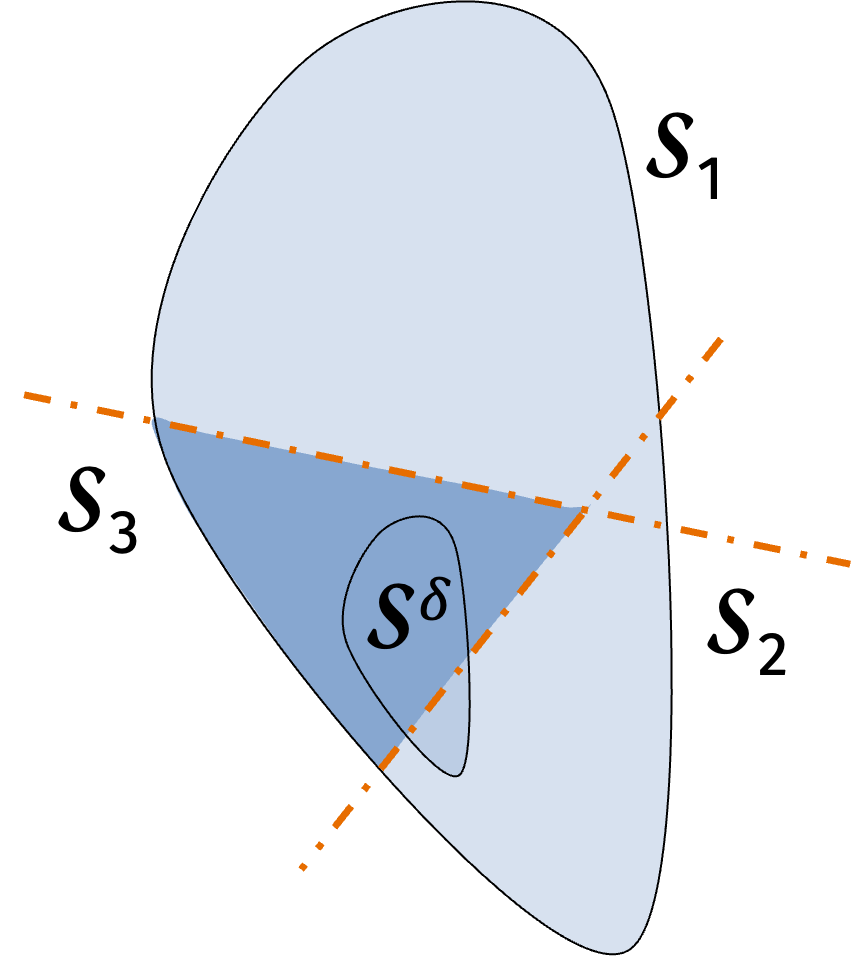
\includegraphics[width=\textwidth]{cut_off.png}
		\end{column}
		\begin{column}{.6\textwidth}
			\vspace{.5em}
			\textbf{Claim:} If we ``chopped off'' at least one point $\bv{y}$ in $\mathcal{S}^\delta$ by the time we reach step $T$ then for some centroid $\bv{c}_1, \ldots, \bv{c}_t$, $f(\bv{c}_t) < 2B\delta$. 
			\vspace{1em}
			
			\textbf{Proof:} 
			\begin{align*}
							2B\delta \geq f(\bv{y}) &\geq f(\bv{c}_t) +  \langle\nabla f(\bv{c}_t), \bv{y}-\bv{c}_t\rangle\\ &> f(\bv{c}_t).
			\end{align*}
		
			Algorithm returns $\argmin_{\bv{c}_i} f(\bv{c}_i)$.

		\end{column}
	\end{columns}
\end{frame}



\begin{frame}[t]
	\frametitle{convergence theorem}
	\begin{theorem}[Center-of-Gravity Convergence]
		Let $f$ be a convex function with values in $[-B,B]$.
		Let $\hat{\bv{x}}$ be the output of the center-of-gravity method run for $T$ iterations. Then:
		\begin{align*}
			f(\hat{\bv{x}}) - f(\bv{x}^*) \leq 2B \left(1-\frac{1}{e}\right)^{T/d} \leq 2B e^{-T/3d}.
		\end{align*}
	\end{theorem}
	If we set $T = O\left(d\log(B/\epsilon)\right)$, then $f(\hat{\bv{x}}) - f(\bv{x}^*) \leq \epsilon$. 

In terms of \emph{gradient-oracle} complexity, this is essentially optimal. So why isn't the algorithm used?
\end{frame}


\begin{frame}[t]
		\frametitle{centroid computation}
		\textbf{In general computing the centroid is hard.} \#P-hard even when when $\mathcal{S}$ is an intersection of half-spaces (a polytope).
		
		Even if the problem isn't hard for your starting convex body $\mathcal{S}$, it likely will become hard for $\mathcal{S} \cap \mathcal{H}_1  \cap \mathcal{H}_2 \cap \mathcal{H}_3 \ldots$. 
		
		So while the \emph{oracle complexity} of dimension-dependent optimization was settled, in the 70s a number of basic questions in terms of \emph{computational complexity.}
\end{frame}

\begin{frame}[t]
	\frametitle{linear programming}
	\textbf{Linear programs} (LPs) are one of the most basic convex constrained, convex optimization problems:
	
	Let $\bv{c}\in \R^d, \bv{b}\in \R^n, \bv{A}\in \R^{n\times d}$ be fixed vectors that define the problem, and let $\bv{x}$ be our variable parameter.
	\begin{align*}
	\min f(\bv{x}) &= \bv{c}^T\bv{x}\\
	\text{subject to } \bv{A}\bv{x} &\geq \bv{b}.
	\end{align*}
	
Think about $\bv{A}\bv{x} \geq \bv{b}$ as a union of half-space constraints:
\begin{align*}
	&\{\bv{x}: \bv{a}_1^T\bv{x} \geq {b}_1 \}\\
		&\{\bv{x}: \bv{a}_2^T\bv{x} \geq {b}_2 \}\\
			&\hspace{2.3em}\vdots\\
			&\{\bv{x}: \bv{a}_n^T\bv{x} \geq {b}_n \}
\end{align*}
	
\end{frame}

\begin{frame}[t]
	\frametitle{linear programming}
	\begin{align*}
		\min f(\bv{x}) &= \bv{c}^T\bv{x}\\
		\text{subject to } \bv{A}\bv{x} &\geq \bv{b}.
	\end{align*}
	
	\begin{center}
		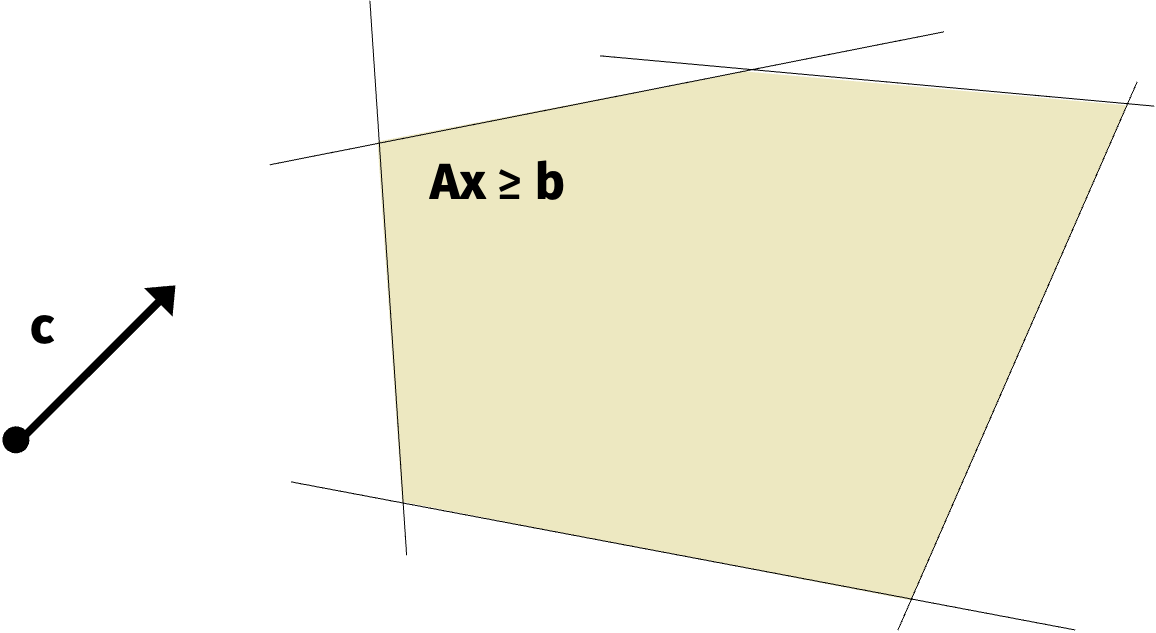
\includegraphics[width=.8\textwidth]{lpexample.png}
	\end{center}
\end{frame}

\begin{frame}
		\frametitle{linear programming applications}
	\begin{itemize}
		\item Classic optimization applications: industrial resource optimization problems were killer app in the 70s.
		\item Robust regression: $\min_{\bv{x}} \|\bv{A} \bv{x} - \bv{b}\|_1$. 
		\item $L1$ constrained regression: $\min_{\bv{x}} \|\bv{x}\|_1$ subject to $\bv{A}\bv{x} = \bv{b}$. Lots of applications in sparse recovery/compressed sensing.
		\item Solve $\min_{\bv{x}}\|\bv{A} \bv{x} - \bv{b}\|_{\infty}$.   
		\item Polynomial time algorithms for Markov Decision Processes. 
		\item \alert{\textbf{Many combinatorial optimization problems can be solved via \emph{LP relaxations}.}}
	\end{itemize}
\end{frame}

\begin{frame}[t]
	\frametitle{linear programming}
	\begin{theorem}[Khachiyan, 1979]
	Assume $n=d$. The \emph{ellipsoid method} solves any linear program with $L$-bit integer valued constraints in $O(n^4L)$ time. I.e. linear programming is in (weakly) polynomial time!
	\end{theorem}
Using a relatively simple center-of-gravity like method!
	\begin{center}
		
\includegraphics[width=\textwidth]{ellipsoidnews.png}
		Front page of New York Times, November 9, 1979.
	\end{center}
\end{frame}

\begin{frame}[t]
	\frametitle{problem simplification}
	\small
		\textbf{Simplifying the problem:}
		Given a convex set $\mathcal{K}$ via access to \emph{separation oracle} $S_\mathcal{K}$ for the set, determine if $\mathcal{K}$ is empty, or otherwise return any point $\bv{x}\in \mathcal{K}$. 
		\vspace{-2em}
		
		\begin{align*}
			\bv{S}_k(\bv{y}) = \begin{cases}
				\emptyset &\text{ if } \bv{y} \in \mathcal{K}. \\
				\text{seperating hyperplane } (\bv{a},c) &\text{ if } \bv{y} \notin \mathcal{K}.
			\end{cases}
		\end{align*}
	
	Let $\mathcal{H} = \{\bv{x}: \bv{a}^T\bv{x} = c\}$.
	\vspace{-1em}
		\begin{center}
			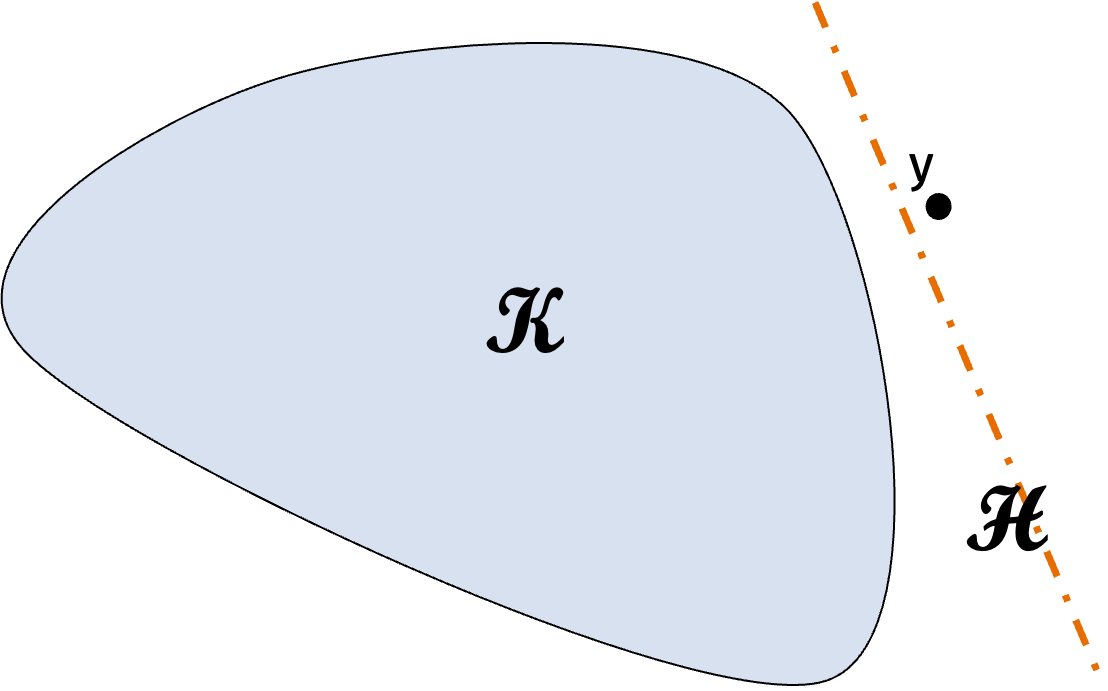
\includegraphics[width=.65\textwidth]{seperationoracle.png}
		\end{center}
	
\end{frame}

\begin{frame}[t]
	\frametitle{separation oracle}
	\textbf{Example:} How would you implement a seperation oracle for a polytope $\{\bv{x}: \bv{A}\bv{x} \geq \bv{b}\}$. 
\end{frame}

\begin{frame}[t]
	\frametitle{from membership to optimization}
	\textbf{Original problem:}
	\begin{align*}
		\min_{\bv{x}} f(\bv{x}) \text{ subject to } \bv{x} \in \mathcal{S} 
	\end{align*}
	How can we reduce to determining if a convex set $\mathcal{K}$ is empty or not?
	
	\textbf{Binary search!} For a convex function $f(\bv{x})$, $\{\bv{x}: f(\bv{x}) \leq c\}$ is convex, and you can get a seperation oracle via the gradient.
	\begin{itemize}
		\item Start with upper bound and lower bounds $u$ and $l$ on optimal solution (can be obtained for many problems). 
		\item Check if the convex set $\mathcal{S} \cap  \{\bv{x}: f(\bv{x}) \leq (u+l)/2\}$ contains a point. 
		\item Update $u = (u+l)/2$ if it does,  $l = (u+l)/2$ if not. 
		\item Continue until $|u-l| \leq \epsilon$. 
	\end{itemize}
	
\end{frame}

\begin{frame}[t]
\frametitle{ellipsoid method sketch}
\textbf{Goal of ellipsoid algorithm:} Solve ``Is $\mathcal{K}$ empty or not?" given a seperation oracle for $\mathcal{K}$ under the assumptions that:
\begin{enumerate}
	\item $\mathcal{K} \subset B(\bv{c}_R, R)$.
		\item If non-empty, $\mathcal{K}$ contains $B(\bv{c}_r, r)$ for some $r < R$. 
\end{enumerate}
\begin{center}
	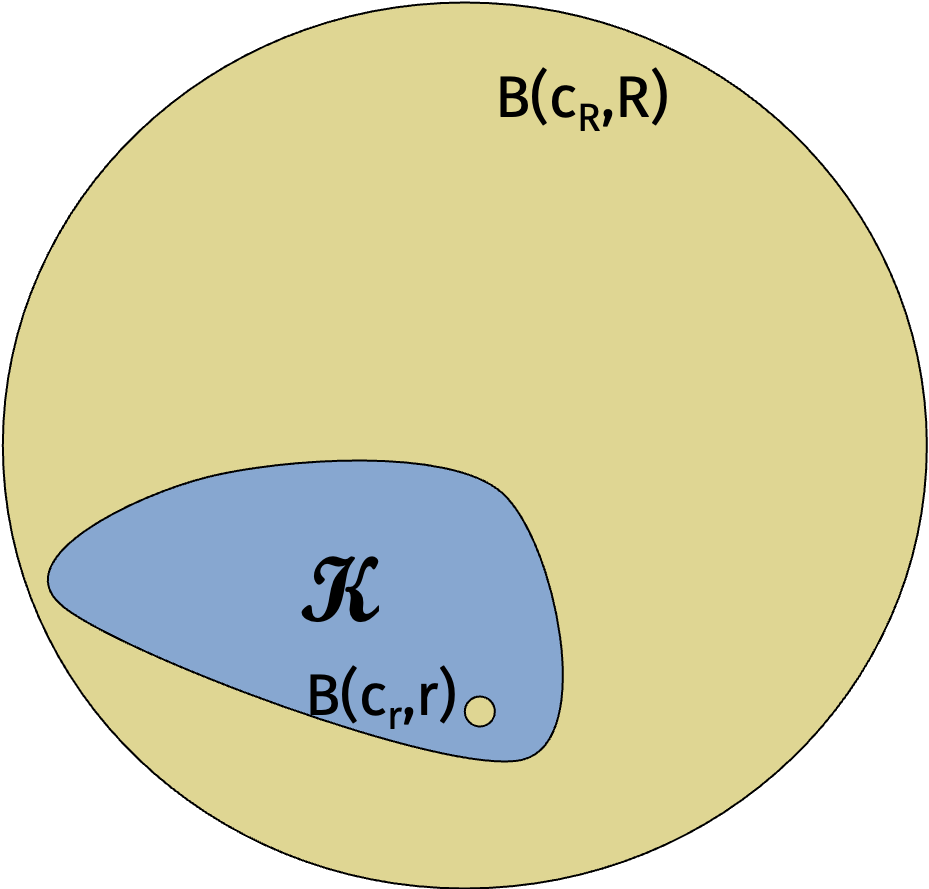
\includegraphics[width=.5\textwidth]{ellipsoid0.png}
\end{center}
	
\end{frame}

\begin{frame}[t]
	\frametitle{ellipsoid method sketch}
	Iterative method similar to center-of-gravity:
	\begin{enumerate}
		\item Check if center $\bv{c}_R$ of $B(\bv{c}_R, R)$ is in $\mathcal{K}$.
		\item If it is, we are done.
		\item  If not, cut search space in half, using seperating hyperplane. 
	\end{enumerate}
	\begin{center}
		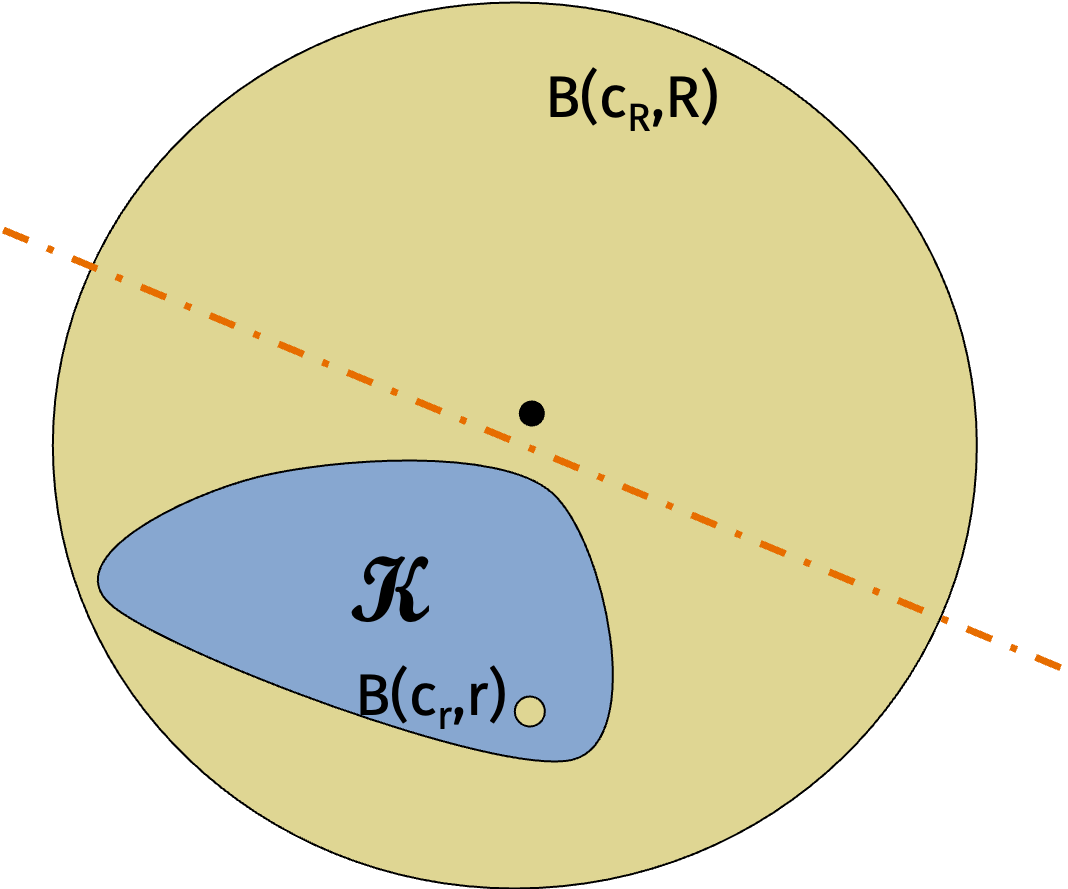
\includegraphics[width=.5\textwidth]{ellipsoid1.png}
	\end{center}
\end{frame}

\begin{frame}[t]
	\frametitle{ellipsoid method sketch}
	\textbf{Key insight:} Before moving on, approximate new search region by something that we can easily compute the centroid of. Specifically an ellipse!!
	\vspace{-1em}
	\begin{center}
		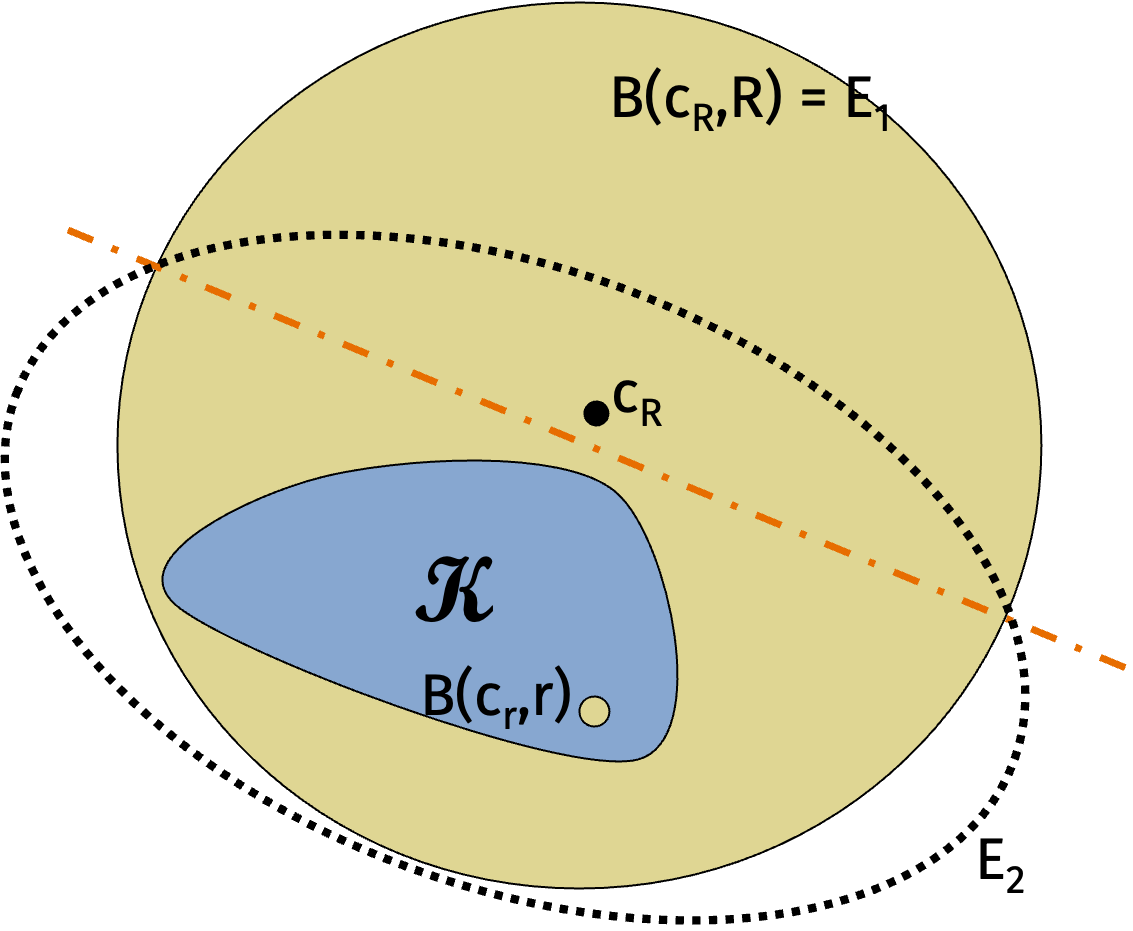
\includegraphics[width=.5\textwidth]{ellipsoid2.png}
	\end{center}
	\vspace{-1em}
Produce a sequence of ellipses that \emph{always contain} $\mathcal{K}$ and decrease in volume: $B(\bv{c}_R, R) = E_1, E_2, \ldots$. Once we get to an ellipse with volume $\leq B(\bv{c}_r, r)$, we know that $\mathcal{K}$ must be empty.
\end{frame}

\begin{frame}
		\frametitle{ellipse}
		An ellipse is a convex set of the form: $\{\bv{x}: \|\bv{A}(\bv{x} - \bv{c})\|_2^2 \leq \alpha\}$ for some constant $c$ and matrix $\bv{A}$. The center-of-mass is  $\bv{c}$. 
		\begin{center}
			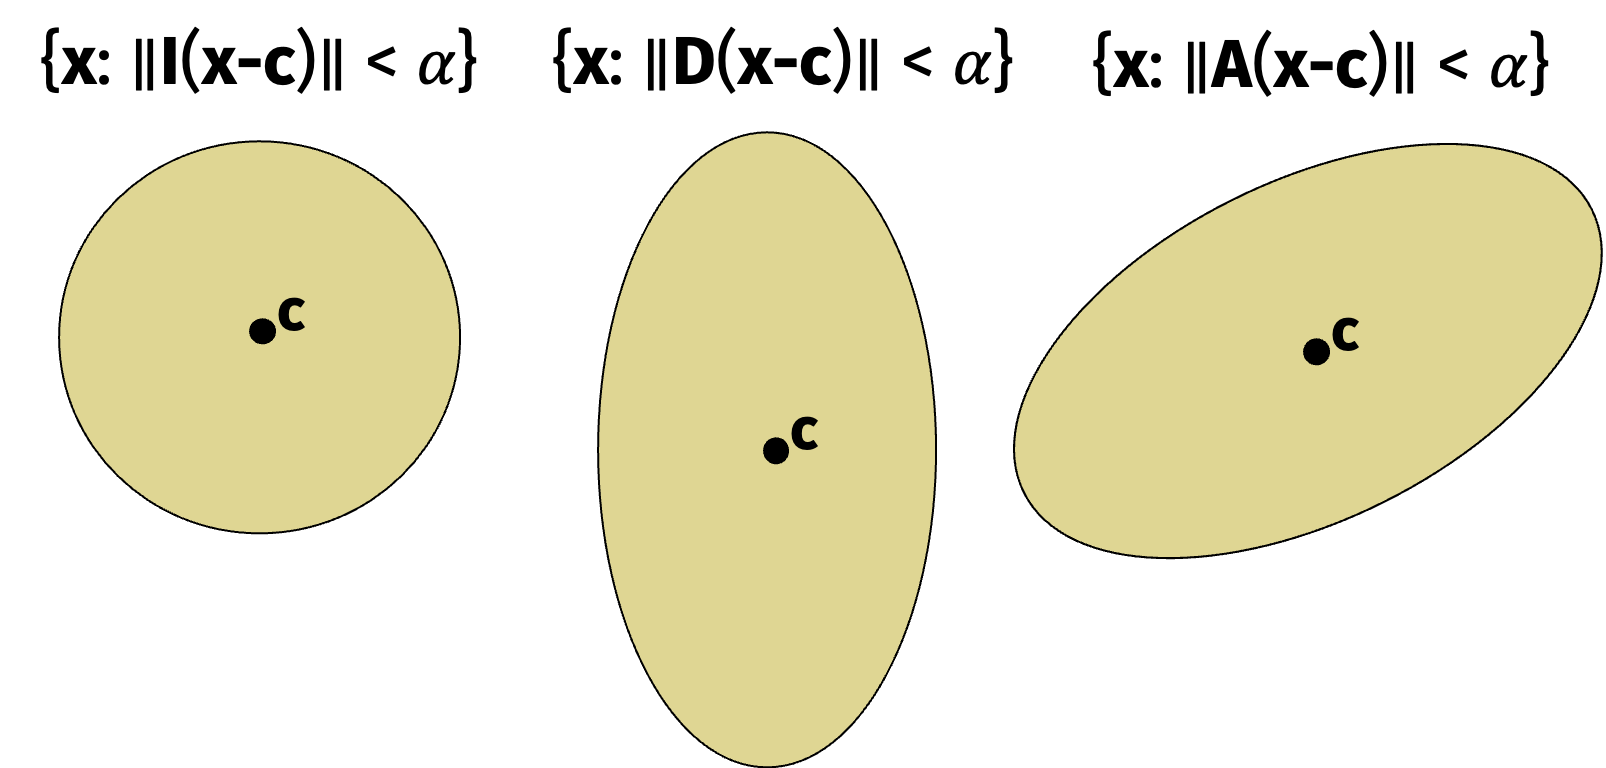
\includegraphics[width=\textwidth]{ellipses.png}
		\end{center}
	
	Often re-parameterized to say that the ellipse is all $\bv{x}$ with $\{\bv{x}: (\bv{x} - \bv{c})^T\bv{Q}^{-1}(\bv{x} - \bv{c})\leq 1\}$
\end{frame}

\begin{frame}
	\frametitle{ellipsoid update}
	There is a closed form solution for the equation of the smallest ellipse containing a given half-ellipse. I.e. let $\bv{E}_i$ have parameters $\bv{Q}_i,\bv{c}_i$ and consider the half-ellipse:
	\begin{align*}
		\bv{E}_i \cap \{\bv{x}: \bv{a}_i^T\bv{x} \leq \bv{a}_i^T\bv{c}_i\}. 
	\end{align*}
Then $\bv{E}_{i+1}$ is the ellipse with parameters:
\begin{align*}
	\bv{Q}_{i+1} &= \frac{d^2}{d^2 - 1}\left(\bv{Q}_{i} - \frac{2}{d+1} \bv{h}\bv{h}^T \right) & \bv{c}_{i+1}& = \bv{c}_{i} - \frac{1}{n+1}\bv{h},
\end{align*}
where $\bv{h} = \sqrt{\bv{a}_i^T\bv{Q}_i\bv{a}_i}\cdot \bv{a}_i$. 
	
\end{frame}


\begin{frame}[t]
	\frametitle{geometric observation}
	\textbf{Claim:} $\vol(E_{i+1}) \leq (1-\frac{1}{2d})\vol(E_i)$.
	
	\textbf{Proof:} Via reduction to the ``isotropic case''. I will post a proof on the course website if you are interested. 
	\vspace{-.5em}
	\begin{center}
		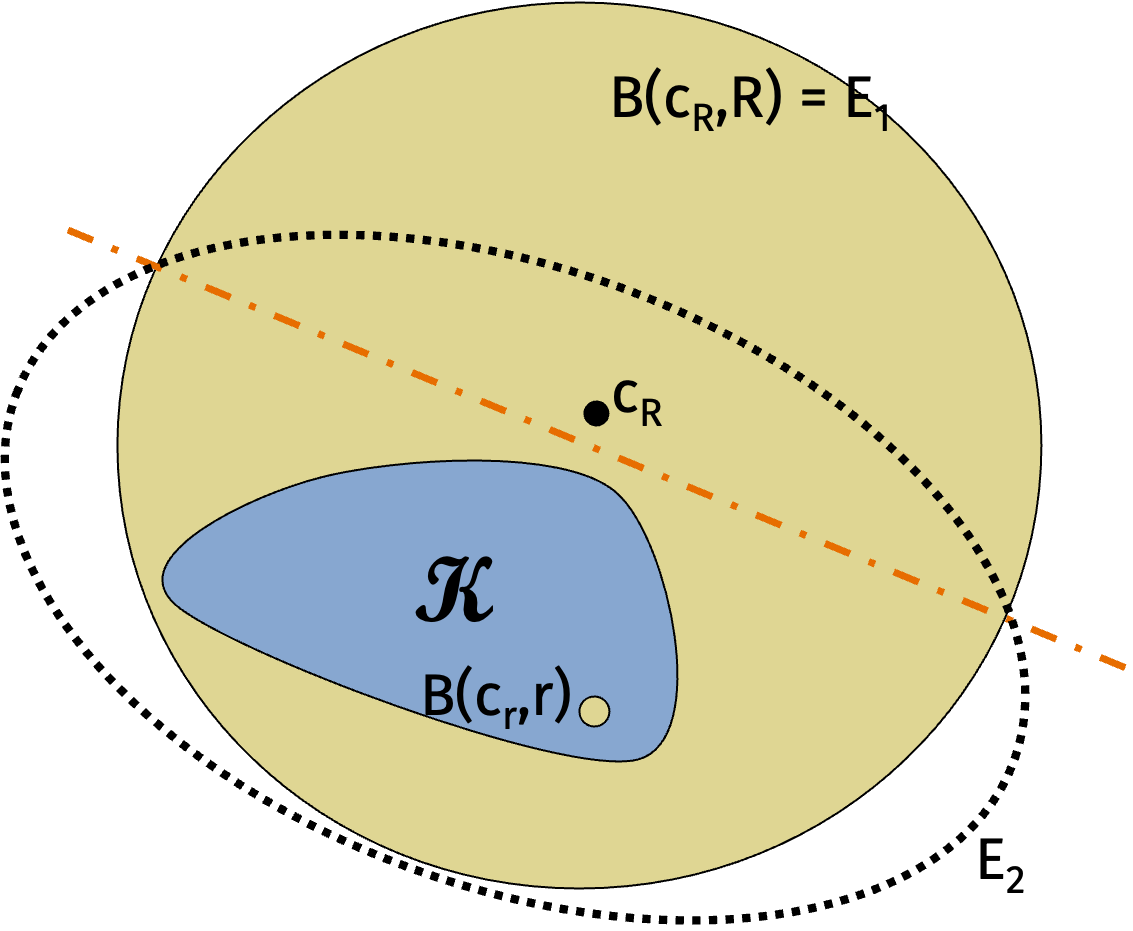
\includegraphics[width=.5\textwidth]{ellipsoid2.png}
	\end{center}
	\vspace{-.5em}
Not as good as the $(1-\frac{1}{e})$ constant-factor volume reduction we got from center-of-gravity, but still very good! 
\end{frame}


\begin{frame}[t]
	\frametitle{geometric observation}
	\textbf{Claim:} $\vol(E_{i+1}) \leq (1-\frac{1}{2d})\vol(E_i)$

	\begin{center}
		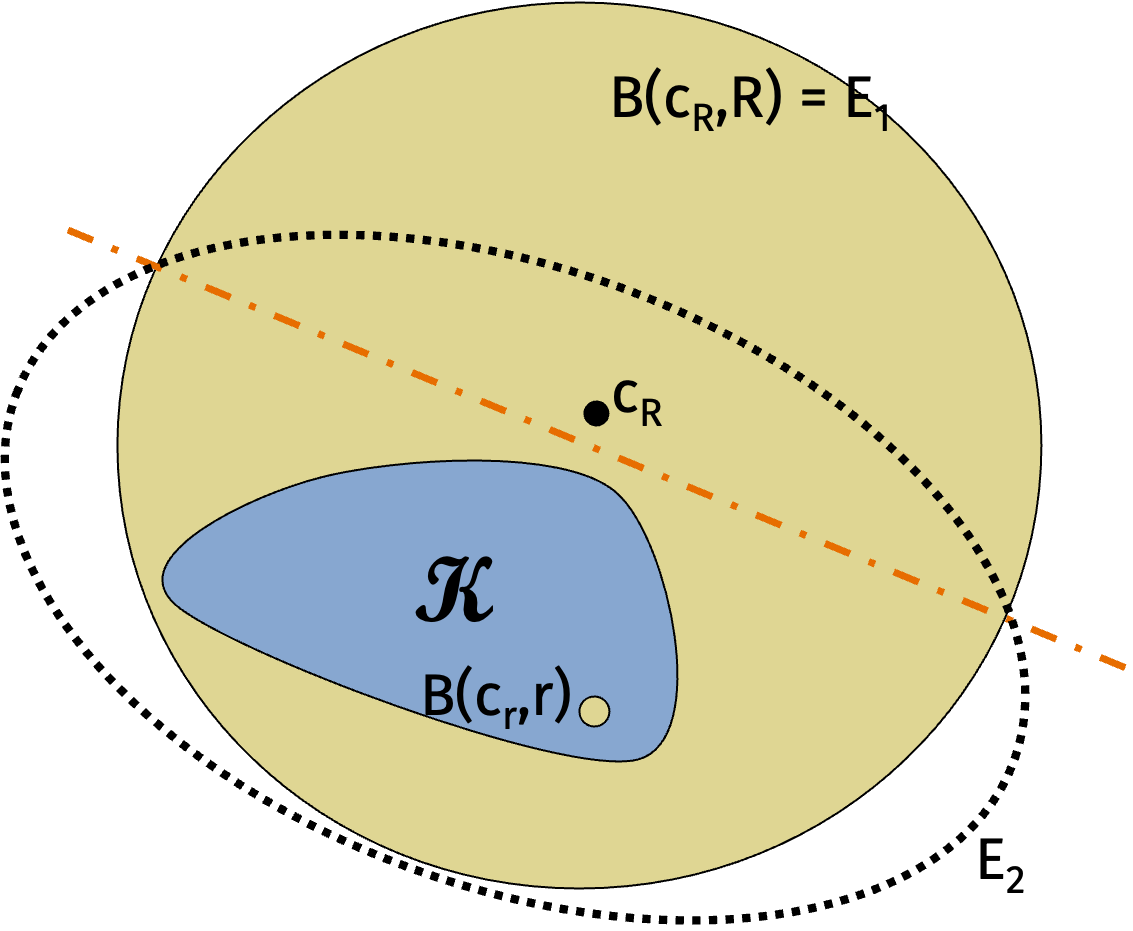
\includegraphics[width=.5\textwidth]{ellipsoid2.png}
	\end{center}
	\begin{center}
		After $O(d)$ iterations, we reduce the volume by a constant.
		
		In total require $O(d^2\log(R/r))$ iterations to solve the problem.
	\end{center}
\end{frame}

\begin{frame}[t]
	\frametitle{ellipsoid for LPs}
	\begin{theorem}[Khachiyan, 1979]
		Assume $n=d$. The \emph{ellipsoid method} solves any linear program with $L$-bit integer valued constraints in $O(n^4L)$ time. I.e. linear programming is in (weakly) polynomial time!
	\end{theorem}
The method works for any convex program. 

For LPs, we have an $O(nd)$ time seperation oracle, and ellipsoid update take $O(d^2)$ time.

 Careful analysis of the binary search method, how to set $B_r$ and $B_R$, etc. leads to the final runtime bound. 
\end{frame}

\begin{frame}[t]
	\frametitle{interior point methods}
	\begin{theorem}[Karmarkar, 1984]
		Assume $n=d$. The \emph{interior point method} solves any linear program with $L$-bit integer valued constraints in $O(n^{3.5}L)$ time. 
	\end{theorem}
	\begin{center}
	
\includegraphics[width=.7\textwidth]{interiornews.png}
	
			Front page of New York Times, November 19, 1984.
	\end{center}
\end{frame}

\begin{frame}[t]
	\frametitle{interior point methods}
	Will post lecture notes on the website (optional reading).
	\begin{center}
			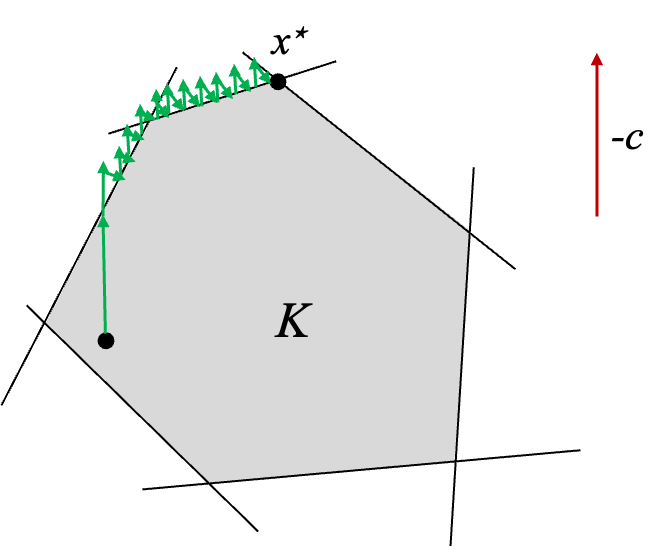
\includegraphics[width=.6\textwidth]{projected_gradient.png}
			
			Projected Gradient Descent Optimization Path
	\end{center}

\end{frame}

\begin{frame}[t]
	\frametitle{interior point methods}
	Will post lecture notes on the website (optional reading).
	\begin{center}
		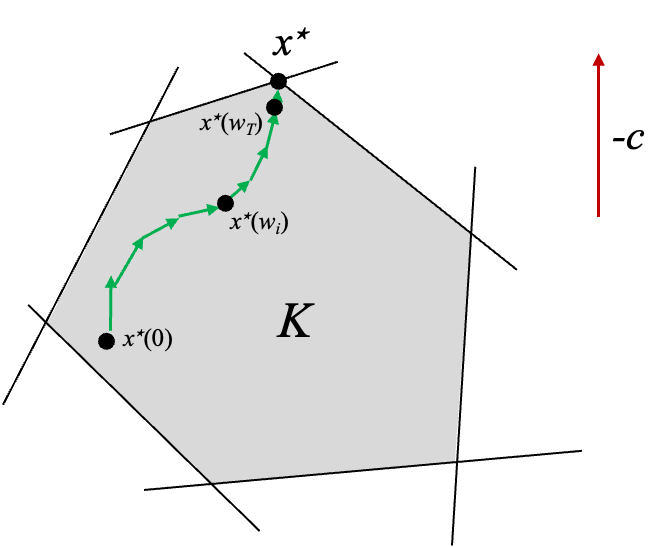
\includegraphics[width=.6\textwidth]{interior_point.png}
		
		Ideal Interior Point Optimization Path
	\end{center}
	
\end{frame}

\begin{frame}[t]
	\frametitle{polynomial time linear programming}
	Both results had a huge impact on the theory of optimization, although at the time neither the ellipsoid method or interior point method were faster than a heuristic known at the Simplex Method. 
	
	These days, improved interior point methods compete with and often outperform simplex. 
	
\end{frame}

\begin{frame}[standout]
	\begin{center}
			\large lp relaxation
		\end{center}
\end{frame}

\begin{frame}
	\frametitle{set cover problem}	
	Given:
	\begin{itemize}
		\item $n$ ground elements $\{1,\ldots,n\}$
		\item $m$ sets $S_1,S_2,\ldots,S_m$ where $S_j \subseteq \{1,\ldots,n\}$
		\item non-negative weights $c_1, \ldots, w_m\geq 0$
	\end{itemize}
	
	\vspace{2em}
	
	Find:
	\begin{align*}
		\min_{Z \subseteq \{1,\ldots,m\}}
		\sum_{j \in Z} c_j
		\hspace{2em}
		\textnormal{ subject to }
		\hspace{2em}
		\cup_{j \in Z} S_j = \{1,\ldots,n\}.
	\end{align*}

\begin{center}
\textbf{\alert{This is an NP-Complete combinatorial optimization problem! Likely impossible to find an efficient \emph{exact} algorithm.}}
\end{center}
\end{frame}

\begin{frame}
	\frametitle{applications}
	\begin{itemize}
		\item Finding efficient sets of test cases for code testing and verification.
		\item Complex employee shift scheduling problems (e.g. in the airline industry).
		\item Motif selection in computational biology.
	\end{itemize}
\end{frame}

\begin{frame}
	\frametitle{application: vertex cover}
	
	Given:
	\begin{itemize}
		\item ground elements are edges
		\item sets are nodes so
		\begin{align*}
			S_j = \{ \textnormal{edges adjacent to
				$j$th node}\}
		\end{align*}
		\item Could have $c_j=1$ for all $j\in 1, \ldots, m$ or could have different costs per node.
	\end{itemize}
	\vspace{2em}
	
	What vertices should we choose so that all
	edges are connected to at least one chosen
	vertex?
\end{frame}

\begin{frame}
	\frametitle{linear programming}
	Let $\mathbf{x} \in \R^m$ be a vector
	of decision variables, $\mathbf{c}$ be a cost vector, and $\mathbf{b} \in \R^n$
	be a vector of constraints. As before a linear program has the form
	the linear programs is:
	\begin{align*}
		\textnormal{Minimize} \hspace{1em}
		\mathbf{c^T x} \hspace{1em}
		&\textnormal{ subject to } \hspace{1em}
		\mathbf{Ax \geq b}, \hspace{1em}
%		\mathbf{x} \geq 0 \hspace{1em}
	\end{align*}
	
	\vspace{2em}	
	
	\textbf{Goal:} Show that set cover can be written as a linear program, except with the additional constraint that $\bv{x}$ is a \emph{binary} random vector. This is called an  \textbf{\alert{integer linear program}}.
\end{frame}

\begin{frame}
	\frametitle{lp for set cover: objective}
	
	Let $x_j = 1$ iff $j \in Z$. $0$ otherwise
	
	The objective is to minimize the sum of weights
	in $Z$:
	
	\begin{align*}
		\min_{Z\subseteq \{1,\ldots,m\}} \sum_{j \in Z} c_j
		\hspace{1em} \Leftrightarrow \hspace{1em}
		\min_{\mathbf{x}} \sum_{j=1}^m c_j x_j
		\hspace{1em} \Leftrightarrow \hspace{1em}
		\min_{\mathbf{x}} \mathbf{c^T x}
	\end{align*}
\end{frame}

\begin{frame}
	\frametitle{lp for set cover: constraint}
	
	The constraint is that $C$
	covers the ground elements. I.e. for all $i \in 1,\dots, n$, we should have:
	
	\begin{align*}
		i \in \cup_{j \in Z} S_j
		\hspace{1.5em} \Leftrightarrow \hspace{1em}
		\sum_{j:i \in S_j}^m x_j \geq 1 
		\hspace{1.5em} \Leftrightarrow \hspace{1em}
		\mathbf{A x \geq c}
	\end{align*}	
	
	\textbf{Question:} What are $\mathbf{A}$ and $\mathbf{b}$?
	
\end{frame}

\begin{frame}
	\frametitle{lp for set cover: statement}
	\begin{align*}
		\textnormal{Minimize} \hspace{1em}
		\mathbf{c^T x} \hspace{1em}
		&\textnormal{ subject to } \hspace{1em}
		\mathbf{Ax \geq b}, \hspace{1em} \bv{x}\in \{0,1\}^m		\\
		\textnormal{Minimize} \hspace{1em}
		\sum_{j=1}^m c_j x_j \hspace{1em}
		&\textnormal{ subject to } \hspace{1em}
		\sum_{j: i \in S_j} x_j \geq 1,  \hspace{1em}  \bv{x}\in \{0,1\}^m
	\end{align*}
	
	Without the constraint $\bv{x}\in \{0,1\}^m$, we can solve  linear program
	in polynomial time with e.g. Interior Point,
	Ellipsoid Method. But we will get a \textbf{\alert{fractional solution}}.
\end{frame}

\begin{frame}
	\frametitle{lp relaxation}
	
	\begin{definition}[Relaxation]
		A linear program (where $\mathbf{x} \in \R^m$)
		is a \textit{relaxation} of an integer program
		(where $\mathbf{x} \in \{0,1\}^m$) if
		\begin{itemize}
			\item a feasible solution to the ILP is
			a feasible solution to the LP and
			\item the value of the feasible solution in
			the ILP has the same value in the LP.
		\end{itemize}
	\end{definition}
	
	\begin{center}
	We always have that $OPT_{LP} \leq OPT_{ILP}$.
	\end{center}
\end{frame}

\begin{frame}
		\frametitle{lp rounding}
		\textbf{Common approach for \emph{approximately} solving ILPs:} 
		
		Find a solution to an LP relaxation for the IP and then ``round'' the solution to be binary or integer. E.g round numbers close to $0$ to $0$, numbers close to $1$ to $1$. Often randomization is used in the rounding process. 
\end{frame}

\begin{frame}
	\frametitle{lp to set cover}
	
	\begin{theorem}
		Let $\mathbf{x^*}$ be optimal solution to LP.
		Define 
		\begin{align*}
			f = \max_{i \in 1,\ldots,n} |\{j: i \in S_j\}|.
		\end{align*}
		\textbf{Rounding procedure:} Put $j \in Z$ if and only if $x^*_j \geq 1/f$.
		
		Then $Z$ is feasible and gives an 
		$f$-approximation to set cover.
	\end{theorem}
	
	\textbf{Question:} What approximation do 
	we get for vertex cover?
\end{frame}

\begin{frame}
	\frametitle{lp to set cover: proof}
	\textbf{Claim:} $C$ is feasible.
	
	Fix $i$. We know
	\begin{align*}
		\sum_{j: i \in S_j} x^*_j \geq 1.
	\end{align*}
	Then
	
	\vspace{10em}
\end{frame}

\begin{frame}
	\frametitle{lp to set cover: proof}
	\textbf{Claim:} $C$ gives an $f$-approximation to set cover.
	
	\begin{align*}
		Cost_{LP} &= \sum_{j=1}^m x_j^* c_j & Cost_{ILP} = \sum_{j\in Z} c_j
	\end{align*}
	
	\vspace{10em}
\end{frame}

\end{document} 








